\documentclass[10pt]{ctexart}
\usepackage{geometry}
\geometry{a4paper, margin=2.5cm}
\usepackage{graphicx}
\usepackage{amsmath, amsfonts}
\usepackage{listings}
\usepackage{xcolor}
\usepackage{caption}
\usepackage{float}
\usepackage{fontspec} % 字体支持
\usepackage{xeCJK}    % 中文支持

% 设置中文字体
\setCJKmainfont{SimHei} % 你可以选择其他字体

\lstset{
    basicstyle=\ttfamily,
    columns=flexible,
    keepspaces=true,
    language=Python,
    showstringspaces=false,
    morekeywords={plt, sns},  % 自定义更多关键词
    backgroundcolor=\color{gray!10},  % 背景色
    keywordstyle=\color{blue},  % 关键词颜色
    stringstyle=\color{red},  % 字符串颜色
    commentstyle=\color{green},  % 注释颜色
    breaklines=true,  % 自动换行
    frame=single,  % 加框
    tabsize=4,  % 设置制表符大小
    showstringspaces=false  % 不显示字符串中的空格
}

\title{\textbf{一次数据处理的尝试}\\[0.5em]
\Large 基于 Online Retail II 数据集的 PCA + 聚类分析}
\author{姓名:李锦源 \quad 学号:20238131022}
\date{}

\begin{document}

\maketitle

\section{项目目标}
本项目旨在完成一次真实的数据归约任务,结合实际数据集进行降维、聚类和可视化操作。我们选用来自 UCI 的“Online Retail II”数据集,并通过主成分分析(PCA)和 KMeans 聚类算法完成降维和客户分群。

\section{数据来源}
\begin{itemize}
    \item \textbf{数据名称}:Online Retail II
    \item \textbf{来源链接}:\url{https://archive.ics.uci.edu/dataset/502/online+retail+ii}
    \item \textbf{简介}:该数据集包含一家英国在线零售商在2010至2011年的交易记录,包括客户ID、国家、商品描述、数量、单价等字段。
\end{itemize}

\section{数据处理流程}

\subsection{数据读取与清洗}
使用 Pandas 读取 Excel 数据,并对缺失值进行删除处理。同时去除 Quantity 和 Price 中的非正值,保证数据质量。

\begin{lstlisting}
data = pd.read_excel('online_retail_II.xlsx', sheet_name='Year 2010-2011')
data.dropna(inplace=True)
features = data[['Quantity', 'Price']]
features = features[(features > 0).all(axis=1)]
\end{lstlisting}

\subsection{数据标准化}
为了避免量纲影响,将数据进行标准化处理。

\begin{lstlisting}
from sklearn.preprocessing import StandardScaler
scaler = StandardScaler()
scaled_data = scaler.fit_transform(features)
\end{lstlisting}

\subsection{维度规约:PCA 降维}
将数据压缩为两个主成分,利于可视化与聚类。

\begin{lstlisting}
from sklearn.decomposition import PCA
pca = PCA(n_components=2)
pca_data = pca.fit_transform(scaled_data)
\end{lstlisting}

\subsection{数量规约:KMeans 聚类}
将客户分群,达到聚类分析与简化数据结构的目的。

\begin{lstlisting}
from sklearn.cluster import KMeans
kmeans = KMeans(n_clusters=3, random_state=42)
clusters = kmeans.fit_predict(scaled_data)
\end{lstlisting}

\subsection{数据可视化}
通过 PCA 主成分作为横纵坐标,聚类标签作为颜色,展示客户分布。

\begin{lstlisting}
df_plot = pd.DataFrame(pca_data, columns=['PC1', 'PC2'])
df_plot['Cluster'] = clusters

plt.figure(figsize=(8, 6))
sns.scatterplot(data=df_plot, x='PC1', y='PC2', hue='Cluster', palette='viridis', s=60)
plt.title('PCA + KMeans 聚类图')
plt.xlabel('主成分1')
plt.ylabel('主成分2')
plt.tight_layout()
plt.savefig('cluster_plot.png', dpi=300)
plt.show()
\end{lstlisting}

可视化结果如下图所示:

\begin{figure}[H]
    \centering
    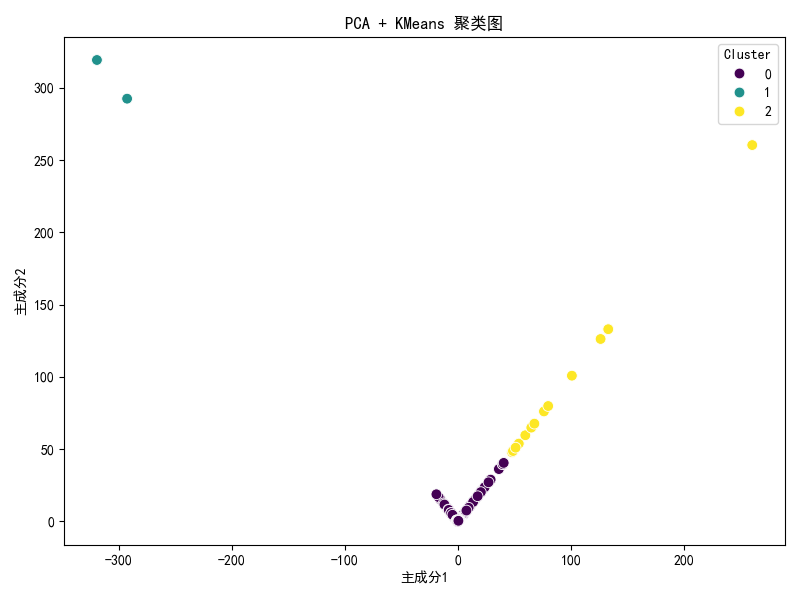
\includegraphics[width=0.7\textwidth]{cluster_plot.png}
    \caption{主成分分析与聚类可视化}
\end{figure}

\section{结果分析}
\begin{itemize}
    \item PCA压缩保留了大部分数据信息,有效简化了数据维度。
    \item KMeans将用户聚为3类,为进一步的用户行为分析提供了基础。
    \item 数据归约使得处理效率大幅提高,同时提升了可视化效果。
\end{itemize}

\section{总结与反思}
通过本次项目,我掌握了数据清洗、标准化、PCA降维、聚类分析与可视化技能,理解了数据归约在实际应用中的价值。Python 的数据科学工具链为高效分析提供了极大便利。

\section*{附录}
\begin{itemize}
    \item Python 源代码:见项目文件
    \item 图像文件:\texttt{cluster\_plot.png}
\end{itemize}

\end{document}
